
\section{Introduction au Prompt Engineering}
\subsection{Concepts fondamentaux}

\begin{frame}[fragile]{Qu'est-ce qu'un prompt ?}
\begin{block}{Définition}
Un \textbf{prompt} est l'instruction textuelle donnée à un modèle d'IA générative pour produire une réponse.
\end{block}

\vspace{0.5cm}

\begin{columns}
\column{0.5\textwidth}
\textbf{Analogie :}
\begin{itemize}
    \item Question à un expert
    \item Commande à un assistant
    \item Spécification d'une tâche
\end{itemize}

\column{0.5\textwidth}
\textbf{Exemple simple :}
\begin{lstlisting}
"Explique-moi la photosynthese"
\end{lstlisting}
\end{columns}

\vspace{0.3cm}
\begin{alertblock}{Point clé}
La qualité du prompt détermine la qualité de la réponse
\end{alertblock}
\end{frame}

\begin{frame}{Les tokens}
\begin{block}{Définition}
Un \textbf{token} est l'unité de base de traitement du texte par le modèle. Un mot peut correspondre à 1 ou plusieurs tokens.
\end{block}

\vspace{0.3cm}

\begin{columns}
\column{0.5\textwidth}
\textbf{Exemples de tokenisation :}
\begin{itemize}
    \item "chat" $\rightarrow$ 1 token
    \item "extraordinaire" $\rightarrow$ 2-3 tokens
    \item "IA" $\rightarrow$ 1 token
    \item "l'intelligence" $\rightarrow$ 2 tokens
\end{itemize}

\column{0.5\textwidth}
\textbf{Pourquoi c'est important ?}
\begin{itemize}
    \item Limite de contexte (ex: 200k tokens)
    \item Coût de l'API
    \item Vitesse de traitement
\end{itemize}
\end{columns}

\vspace{0.3cm}
\begin{exampleblock}{Règle approximative}
1 token $\simeq$  0.75 mot en français | 100 tokens $\simeq$ 75 mots
\end{exampleblock}
\end{frame}

\begin{frame}{La température}
\begin{block}{Définition}
La \textbf{température} est un paramètre (0 à 1+) qui contrôle le caractère aléatoire/créatif des réponses du modèle.
\end{block}

\vspace{0.3cm}

\begin{center}
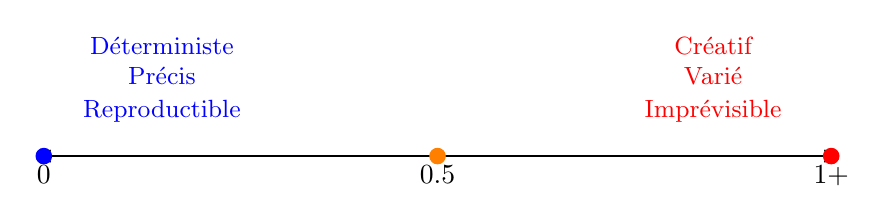
\begin{tikzpicture}
    \draw[<->,thick] (0,0) -- (10,0);
    \node[below] at (0,0) {0};
    \node[below] at (5,0) {0.5};
    \node[below] at (10,0) {1+};
    
    \node[above,text width=3cm,align=center] at (1.5,0.3) {\small \textcolor{blue}{Déterministe\\Précis\\Reproductible}};
    \node[above,text width=3cm,align=center] at (8.5,0.3) {\small \textcolor{red}{Créatif\\Varié\\Imprévisible}};
    
    \fill[blue] (0,0) circle (3pt);
    \fill[orange] (5,0) circle (3pt);
    \fill[red] (10,0) circle (3pt);
\end{tikzpicture}
\end{center}

\vspace{0.3cm}

\begin{columns}
\column{0.5\textwidth}
\textbf{Température basse (0-0.3) :}
\begin{itemize}
    \item Analyse de données
    \item Code informatique
    \item Traduction technique
\end{itemize}

\column{0.5\textwidth}
\textbf{Température haute (0.7-1) :}
\begin{itemize}
    \item Écriture créative
    \item Brainstorming
    \item Génération d'idées
\end{itemize}
\end{columns}
\end{frame}

\begin{frame}{Le contexte}
\begin{block}{Définition}
Le \textbf{contexte} est l'ensemble des informations fournies au modèle : historique de conversation, documents, instructions, etc.
\end{block}

\vspace{0.3cm}

\begin{columns}
\column{0.5\textwidth}
\textbf{Fenêtre de contexte :}
\begin{itemize}
    \item GPT-4: 128k tokens
    \item Claude 3: 200k tokens
    \item Gemini 1.5: 1M tokens
\end{itemize}

\column{0.5\textwidth}
\textbf{Types de contexte :}
\begin{itemize}
    \item Conversation précédente
    \item Documents joints
    \item Instructions système
    \item Exemples fournis
\end{itemize}
\end{columns}

\vspace{0.3cm}

\begin{exampleblock}{Exemple}
\textit{"Selon le document PDF joint, quelles sont les recommandations concernant..."} \\
$\rightarrow$ Le PDF fait partie du contexte
\end{exampleblock}
\end{frame}

\begin{frame}[fragile]{Le prompt système (System Prompt)}
\begin{block}{Définition}
Le \textbf{prompt système} est une instruction permanente qui définit le comportement global du modèle, invisible pour l'utilisateur final.
\end{block}

\vspace{0.3cm}

\begin{columns}
\column{0.55\textwidth}
\textbf{Fonction :}
\begin{itemize}
    \item Définir le rôle de l'IA
    \item Établir des contraintes
    \item Fixer le style de réponse
    \item Définir des règles éthiques
\end{itemize}

\column{0.45\textwidth}
\begin{lstlisting}[basicstyle=\ttfamily\tiny]
Tu es un assistant medical 
specialise en cardiologie.
Tu dois toujours :
- Etre precis
- Citer tes sources
- Rappeler de consulter 
  un medecin
\end{lstlisting}
\end{columns}

\vspace{0.3cm}

\begin{alertblock}{Important}
Le prompt système n'est généralement pas modifiable par l'utilisateur dans les applications finales (ChatGPT, Claude, etc.)
\end{alertblock}
\end{frame}

\begin{frame}{Rôle et tâche}
\begin{columns}
\column{0.5\textwidth}
\begin{block}{Le rôle}
Identité ou expertise attribuée au modèle
\end{block}

\textbf{Exemples :}
\begin{itemize}
    \item "Tu es un professeur de physique"
    \item "Agis comme un expert en cybersécurité"
    \item "Tu es un coach sportif"
\end{itemize}

\vspace{0.3cm}
\textbf{Impact :}
\begin{itemize}
    \item \textcolor{green}{\faCheck} Vocabulaire adapté
    \item \textcolor{green}{\faCheck} Angle d'approche pertinent
    \item \textcolor{green}{\faCheck} Niveau d'expertise cohérent
\end{itemize}

\column{0.5\textwidth}
\begin{block}{La tâche}
Action concrète à accomplir
\end{block}

\textbf{Exemples :}
\begin{itemize}
    \item "Résume ce document"
    \item "Crée un plan de cours"
    \item "Analyse ces données"
\end{itemize}

\vspace{0.3cm}
\textbf{Spécificité :}
\begin{itemize}
    \item \textcolor{red}{\faTimes} "Aide-moi avec Python"
    \item \textcolor{green}{\faCheck} "Écris une fonction Python qui calcule la moyenne d'une liste"
\end{itemize}
\end{columns}

\vspace{0.3cm}
\begin{exampleblock}{Combinaison efficace}
\textbf{Rôle} : "Tu es un statisticien" + \textbf{Tâche} : "Analyse ce dataset et identifie les corrélations significatives"
\end{exampleblock}
\end{frame}

\begin{frame}{Les hallucinations}
\begin{block}{Définition}
Une \textbf{hallucination} se produit quand le modèle génère des informations plausibles mais factuellement incorrectes ou inventées.
\end{block}

\vspace{0.3cm}

\begin{columns}
\column{0.5\textwidth}
\textbf{Types d'hallucinations :}
\begin{itemize}
    \item Faits inventés
    \item Dates erronées
    \item Citations fictives
    \item Références inexistantes
    \item Statistiques imaginaires
\end{itemize}

\column{0.5\textwidth}
\textbf{Causes :}
\begin{itemize}
    \item Données d'entraînement limitées
    \item Sur-généralisation
    \item Pression pour répondre
    \item Ambiguïté de la question
\end{itemize}
\end{columns}

\vspace{0.3cm}

\begin{alertblock}{Exemple d'hallucination}
Question : "Qui a gagné le prix Nobel de littérature en 2025 ?" \\
Réponse hallucinnée : "Le prix a été attribué à Jean Dupont pour son roman 'Les Ombres du temps'"
\end{alertblock}

\begin{exampleblock}{Mitigation}
Demander des sources, vérifier les faits critiques, utiliser température basse pour les faits
\end{exampleblock}
\end{frame}

\begin{frame}[fragile]{La chaîne de pensée (Chain-of-Thought)}
\begin{block}{Définition}
La \textbf{chaîne de pensée} est une technique qui encourage le modèle à décomposer son raisonnement en étapes intermédiaires explicites.
\end{block}

\vspace{0.3cm}

\begin{columns}
\column{0.48\textwidth}
\textbf{Sans chaîne de pensée :}
\begin{lstlisting}[basicstyle=\ttfamily\scriptsize]
Q: Si un train part a 13h 
et roule 2h30 a 80km/h, 
quelle distance parcourt-il?

R: 200 km
\end{lstlisting}

\column{0.48\textwidth}
\textbf{Avec chaîne de pensée :}
\begin{lstlisting}[basicstyle=\ttfamily\scriptsize]
Q: [meme question]
Raisonne etape par etape.

R: Etape 1: Temps = 2h30 
           = 2.5 heures
Etape 2: Distance = vitesse 
         x temps
Etape 3: 80 x 2.5 = 200 km
Reponse: 200 km
\end{lstlisting}
\end{columns}

\vspace{0.3cm}

\begin{exampleblock}{Phrases déclencheuses}
"Raisonne étape par étape" | "Pense à haute voix" | "Décompose ton raisonnement" | "Explique ta démarche"
\end{exampleblock}

\textbf{Avantages :} \textcolor{green}{\faCheck} Meilleure précision \quad \textcolor{green}{\faCheck} Raisonnement vérifiable \quad \textcolor{green}{\faCheck} Identification des erreurs
\end{frame}


\begin{frame}{Architecture des systèmes d'IA générative}
\begin{center}
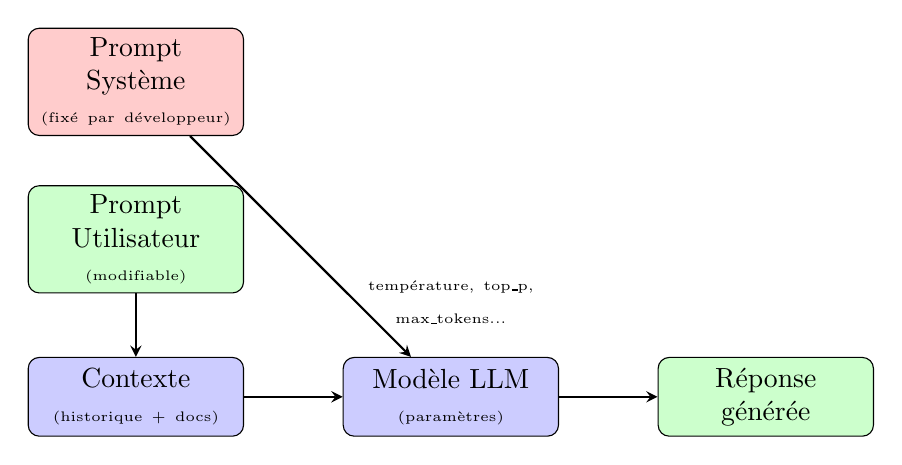
\begin{tikzpicture}[node distance=1.5cm, auto]
    % Styles
    \tikzstyle{block} = [rectangle, draw, fill=blue!20, text width=2.5cm, text centered, rounded corners, minimum height=1cm]
    \tikzstyle{hidden} = [rectangle, draw, fill=red!20, text width=2.5cm, text centered, rounded corners, minimum height=1cm]
    \tikzstyle{user} = [rectangle, draw, fill=green!20, text width=2.5cm, text centered, rounded corners, minimum height=1cm]
    \tikzstyle{arrow} = [thick,->,>=stealth]
    
    % Nodes
    \node [hidden] (system) {Prompt Système\\{\tiny (fixé par développeur)}};
    \node [user, below of=system, node distance=2cm] (user) {Prompt Utilisateur\\{\tiny (modifiable)}};
    \node [block, below of=user, node distance=2cm] (context) {Contexte\\{\tiny (historique + docs)}};
    \node [block, right of=context, node distance=4cm] (model) {Modèle LLM\\{\tiny (paramètres)}};
    \node [user, right of=model, node distance=4cm] (output) {Réponse générée};
    
    % Arrows
    \draw [arrow] (system) -- (model);
    \draw [arrow] (user) -- (context);
    \draw [arrow] (context) -- (model);
    \draw [arrow] (model) -- (output);
    
    % Labels
    \node [above of=model, node distance=1.2cm, text width=3cm, align=center] {\tiny température, top\_p, max\_tokens...};
\end{tikzpicture}
\end{center}

\vspace{0.3cm}

\begin{itemize}
    \item \textcolor{red}{Zone rouge} : Contrôlée par les développeurs de l'application
    \item \textcolor{green}{Zone verte} : Accessible à l'utilisateur final
    \item \textcolor{blue}{Zone bleue} : Géré automatiquement par le système
\end{itemize}
\end{frame}


\section{Bonnes pratiques}

\begin{frame}[fragile]{Principe 1 : Clarté et spécificité}
\begin{columns}
\column{0.48\textwidth}
\begin{alertblock}{\textcolor{red}{\faTimes} Prompt vague}
\begin{lstlisting}[basicstyle=\ttfamily\tiny]
Parle-moi de Python
\end{lstlisting}
\end{alertblock}

{\footnotesize
    \textbf{Problèmes :}
    \begin{itemize}
        \item Trop général
        \item Objectif flou
        \item Réponse imprévisible
    \end{itemize}

    \vspace{0.3cm}

    \textbf{Résultat :}
    \begin{itemize}
        \item Historique du langage ?
        \item Syntaxe de base ?
        \item Bibliothèques populaires ?
        \item Comparaison avec d'autres langages ?
    \end{itemize}
}

\column{0.48\textwidth}
\begin{exampleblock}{\textcolor{green}{\faCheck} Prompt spécifique}
\begin{lstlisting}[basicstyle=\ttfamily\tiny]
Explique comment utiliser les 
list comprehensions en Python 
pour filtrer une liste de nombres 
et ne garder que les pairs. 
Fournis 2 exemples avec des 
commentaires.
\end{lstlisting}
\end{exampleblock}

{\footnotesize

    \textbf{Forces :}
    \begin{itemize}
        \item Sujet précis (list comprehensions)
        \item Tâche claire (filtrer les pairs)
        \item Format demandé (2 exemples commentés)
    \end{itemize}

    \vspace{0.3cm}

    \textbf{Résultat :}
    \begin{itemize}
        \item Réponse ciblée et utile
        \item Exemples pratiques
        \item Gain de temps
    \end{itemize}
}
\end{columns}

\end{frame}



\begin{frame}[fragile]{Principe 2 : Donner du contexte}
\begin{columns}
\column{0.48\textwidth}
\begin{alertblock}{\textcolor{red}{\faTimes} Sans contexte}
\begin{lstlisting}[basicstyle=\ttfamily\tiny]
Explique-moi la regression 
lineaire
\end{lstlisting}
\end{alertblock}

{\footnotesize

\textbf{Problème :}
\begin{itemize}
    \item Niveau d'expertise inconnu
    \item Objectif d'apprentissage flou
    \item Risque d'explications inadaptées
\end{itemize}
}

\column{0.48\textwidth}
\begin{exampleblock}{\textcolor{green}{\faCheck} Avec contexte}
\begin{lstlisting}[basicstyle=\ttfamily\tiny]
Je suis etudiant en premiere 
annee de medecine et j'apprends 
les statistiques pour analyser 
des donnees cliniques. 
Explique-moi la regression 
lineaire avec un exemple medical 
simple, sans formules mathematiques 
complexes.
\end{lstlisting}
\end{exampleblock}

{\footnotesize

\textbf{Forces :}
\begin{itemize}
    \item Public ciblé (étudiant médecine)
    \item Cas d'usage (données cliniques)
    \item Contraintes claires (pas de maths complexes)
\end{itemize}
}

\end{columns}

\vspace{0.3cm}

{\footnotesize
\begin{center}
    \textbf{Qui ?} \textbf{Quoi ?} \textbf{Pourquoi ?} \textbf{Comment ?}
\end{center}
}
\end{frame}

\begin{frame}[fragile]{Principe 3 : Utiliser des exemples (Few-Shot Learning)}
\begin{columns}
\column{0.48\textwidth}
\begin{alertblock}{\textcolor{red}{\faTimes} Zero-shot}
\begin{lstlisting}[basicstyle=\ttfamily\tiny]
Classe ces phrases selon leur 
sentiment : positif, negatif 
ou neutre.

"Ce restaurant est excellent"
\end{lstlisting}
\end{alertblock}

\textbf{Résultat incertain}

\column{0.48\textwidth}
\begin{exampleblock}{\textcolor{green}{\faCheck} Few-shot (avec exemples)}
\begin{lstlisting}[basicstyle=\ttfamily\tiny]
Classe ces phrases selon leur 
sentiment.

Exemples:
"J'adore ce film!" -> positif
"Service deplorable" -> negatif  
"Le ciel est bleu" -> neutre

A toi:
"Ce restaurant est excellent"
\end{lstlisting}
\end{exampleblock}

\textbf{Résultat : positif} \checkmark
\end{columns}

\vspace{0.3cm}

{\footnotesize
    \textbf{Principe :}
    \medskip
    Fournir 2-5 exemples illustrant le format, le style ou la logique attendus. Le modèle apprend par analogie.

    \textbf{Cas d'usage :} Classification, transformation de format, génération structurée, tâches avec conventions spécifiques
}
\end{frame}

\begin{frame}[fragile]{Principe 4 : Structurer la demande}
\begin{columns}
\column{0.48\textwidth}
\begin{alertblock}{\textcolor{red}{\faTimes} Prompt non structuré}
\begin{lstlisting}[basicstyle=\ttfamily\tiny]
J'ai des donnees de patients 
avec age, poids, tension et je 
veux savoir s'il y a des liens 
et fais-moi un resume et aussi 
des graphiques si possible et 
explique comment faire l'analyse
\end{lstlisting}
\end{alertblock}

{\footnotesize
    \textbf{Problèmes :}
    \begin{itemize}
        \item Plusieurs demandes mélangées
        \item Ordre flou
        \item Difficile à suivre
    \end{itemize}
}

\column{0.48\textwidth}
\begin{exampleblock}{\textcolor{green}{\faCheck} Prompt structuré}
\begin{lstlisting}[basicstyle=\ttfamily\tiny]
Contexte: Dataset medical avec 
age, poids, tension arterielle.

Tache:
1. Analyse les correlations
2. Identifie les relations 
   significatives
3. Resume les findings en 3 points
4. Suggere 2 visualisations 
   pertinentes

Format: Pour chaque etape, 
explique ta demarche.
\end{lstlisting}
\end{exampleblock}

{\footnotesize

    \textbf{Forces :}
    \begin{itemize}
        \item Étapes numérotées
        \item Priorités claires
        \item Format défini
    \end{itemize}
}

\end{columns}

\vspace{0.3cm}

{\footnotesize

    \textbf{Techniques de structuration :}

    \textbf{Sections :} Contexte,  Tâche,  Format,  Contraintes

    \textbf{Séparateurs :} --- ou === pour délimiter
}
\end{frame}

\begin{frame}{Principe 5 : Itération et raffinement}
\textbf{Le prompt engineering est un processus itératif}

\vspace{0.3cm}

\begin{center}
Prompt initial $\rightarrow$ Tester $\rightarrow$ Évaluer $\rightarrow$ Raffiner
\end{center}

\vspace{0.3cm}

\begin{columns}
\column{0.5\textwidth}
\textbf{Signaux de problème :}
\begin{itemize}
    \item Réponse hors-sujet
    \item Trop vague ou trop détaillée
    \item Format incorrect
    \item Hallucinations
    \item Ton inapproprié
\end{itemize}

\column{0.5\textwidth}
\textbf{Actions correctives :}
\begin{itemize}
    \item Ajouter du contexte
    \item Préciser le format
    \item Inclure des exemples
    \item Demander chaîne de pensée
    \item Simplifier la demande
\end{itemize}
\end{columns}

\vspace{0.3cm}

\begin{exampleblock}{Conseil pratique}
Gardez une trace des prompts qui fonctionnent bien pour les réutiliser et les adapter
\end{exampleblock}
\end{frame}

\begin{frame}[fragile]{Principe 6 : Définir le rôle et le format}
\begin{columns}
\column{0.48\textwidth}
\begin{alertblock}{\textcolor{red}{\faTimes} Sans rôle ni format}
\begin{lstlisting}[basicstyle=\ttfamily\tiny]
Explique comment fonctionne 
une IRM
\end{lstlisting}
\end{alertblock}

\textbf{Résultat possible :}
\begin{itemize}
    \item Explication technique complexe
    \item Jargon médical
    \item Pas de structure claire
\end{itemize}

\column{0.48\textwidth}
\begin{exampleblock}{\textcolor{green}{\faCheck} Avec rôle et format}
\begin{lstlisting}[basicstyle=\ttfamily\tiny]
Tu es un vulgarisateur scientifique 
pour le grand public.

Explique comment fonctionne une IRM 
en 3 paragraphes courts:
1. Principe de base (sans formules)
2. Deroulement de l'examen
3. Applications medicales courantes

Utilise des analogies du quotidien.
\end{lstlisting}
\end{exampleblock}

\textbf{Résultat :}
\begin{itemize}
    \item Langage accessible
    \item Structure claire
    \item Analogies pertinentes
\end{itemize}
\end{columns}

\vspace{0.3cm}

\end{frame}


\section{Avantages et limites}

\begin{frame}{Avantages du prompt engineering}
\begin{columns}
\column{0.5\textwidth}

{\footnotesize
    \textbf{Productivité :}
    \begin{itemize}
        \item \textcolor{green}{\faCheck} Accélération des tâches répétitives
        \item \textcolor{green}{\faCheck} Automatisation de l'écriture
        \item \textcolor{green}{\faCheck} Génération de code rapide
        \item \textcolor{green}{\faCheck} Recherche et synthèse efficaces
    \end{itemize}

    \vspace{0.3cm}

    \textbf{Accessibilité :}
    \begin{itemize}
        \item \textcolor{green}{\faCheck} Pas besoin de coder
        \item \textcolor{green}{\faCheck} Interface naturelle (langage)
        \item \textcolor{green}{\faCheck} Adaptatif au niveau utilisateur
    \end{itemize}
}

\column{0.5\textwidth}

{\footnotesize
    \textbf{Créativité :}
    \begin{itemize}
        \item \textcolor{green}{\faCheck} Brainstorming efficace
        \item \textcolor{green}{\faCheck} Exploration d'idées
        \item \textcolor{green}{\faCheck} Génération de variantes
        \item \textcolor{green}{\faCheck} Perspectives multiples
    \end{itemize}

    \vspace{0.3cm}

    \textbf{Apprentissage :}
    \begin{itemize}
        \item \textcolor{green}{\faCheck} Tuteur personnalisé 24/7
        \item \textcolor{green}{\faCheck} Explications adaptées
        \item \textcolor{green}{\faCheck} Exemples à la demande
    \end{itemize}
}
\end{columns}

\end{frame}

\begin{frame}{Limites et risques}
\begin{columns}
    
\column{0.5\textwidth}

{\footnotesize

    \textbf{Fiabilité :}
    \begin{itemize}
        \item \textcolor{red}{\faTimes} Hallucinations possibles
        \item \textcolor{red}{\faTimes} Erreurs factuelles
        \item \textcolor{red}{\faTimes} Sources non vérifiables
        \item \textcolor{red}{\faTimes} Biais des données d'entraînement
    \end{itemize}

    \vspace{0.3cm}

    \textbf{Compréhension limitée :}
    \begin{itemize}
        \item \textcolor{red}{\faTimes} Pas de vraie compréhension
        \item \textcolor{red}{\faTimes} Contexte limité
        \item \textcolor{red}{\faTimes} Raisonnement parfois défaillant
    \end{itemize}
}

\column{0.5\textwidth}

{\footnotesize

    \textbf{Dépendances :}
    \begin{itemize}
        \item \textcolor{red}{\faTimes} Risque de sur-dépendance
        \item \textcolor{red}{\faTimes} Atrophie des compétences
        \item \textcolor{red}{\faTimes} Perte de pensée critique
    \end{itemize}

    \vspace{0.3cm}

    \textbf{Considérations éthiques :}
    \begin{itemize}
        \item \textcolor{red}{\faTimes} Propriété intellectuelle
        \item \textcolor{red}{\faTimes} Confidentialité des données
        \item \textcolor{red}{\faTimes} Détection possible du contenu IA
        \item \textcolor{red}{\faTimes} Usage académique réglementé
    \end{itemize}
}
\end{columns}

\vspace{0.3cm}

\begin{block}{Règle d'or}
    \medskip
    \textbf{L'IA assiste, l'humain valide et décide}. Toujours vérifier les informations critiques.
\end{block}
\end{frame}

\begin{frame}{Quand utiliser (ou non) l'IA générative ?}
\begin{columns}
\column{0.5\textwidth}
\begin{block}{Cas d'usage appropriés}
\begin{itemize}
    \item[\textcolor{green}{\faCheck}] Brouillons et premières versions
    \item[\textcolor{green}{\faCheck}] Reformulation et résumés
    \item[\textcolor{green}{\faCheck}] Génération d'idées
    \item[\textcolor{green}{\faCheck}] Code de base / prototypes
    \item[\textcolor{green}{\faCheck}] Traduction
    \item[\textcolor{green}{\faCheck}] Explication de concepts
    \item[\textcolor{green}{\faCheck}] Analyse de données (avec vérif.)
\end{itemize}
\end{block}

\column{0.5\textwidth}
\begin{alertblock}{Cas à éviter}
\begin{itemize}
    \item[\textcolor{red}{\faTimes}] Décisions médicales critiques
    \item[\textcolor{red}{\faTimes}] Conseils juridiques définitifs
    \item[\textcolor{red}{\faTimes}] Calculs financiers précis
    \item[\textcolor{red}{\faTimes}] Citations académiques
    \item[\textcolor{red}{\faTimes}] Données personnelles sensibles
    \item[\textcolor{red}{\faTimes}] Remplacement total de l'expertise
\end{itemize}
\end{alertblock}
\end{columns}

\vspace{0.3cm}

\begin{block}{Principe de validation}
Plus la décision est critique, plus la vérification humaine experte est nécessaire
\end{block}
\end{frame}

% % \section{Exercices pratiques}

% % \begin{frame}[fragile]{Exercice 1 : Améliorer un prompt}
% % \textbf{Objectif :} Transformer un prompt vague en prompt efficace

% % \vspace{0.3cm}

% % \begin{alertblock}{Prompt de départ (faible)}
% % \begin{lstlisting}
% % Parle-moi des antibiotiques
% % \end{lstlisting}
% % \end{alertblock}

% % \vspace{0.3cm}

% % \textbf{Consignes :}
% % \begin{enumerate}
% %     \item Ajoutez un contexte (ex: étudiant en pharmacie, patient curieux...)
% %     \item Définissez un rôle pour l'IA
% %     \item Précisez la tâche exacte
% %     \item Spécifiez le format de réponse
% %     \item Ajoutez 2-3 contraintes
% % \end{enumerate}

% % \vspace{0.3cm}

% % \textbf{Temps :} 10 minutes \\
% % \textbf{Travail :} Individuel puis mise en commun
% % \end{frame}

% % \begin{frame}[fragile]{Exercice 1 : Exemple de solution}
% % \begin{exampleblock}{Prompt amélioré}
% % \begin{lstlisting}[basicstyle=\ttfamily\scriptsize]
% % Contexte: Je suis etudiant en 2eme annee de pharmacie et je 
% % prepare un expose sur les antibiotiques.

% % Role: Tu es un professeur de microbiologie pharmaceutique.

% % Tache: Explique les mecanismes d'action des principales classes 
% % d'antibiotiques (beta-lactamines, aminoglycosides, quinolones).

% % Format: 
% % - Introduction generale (3 lignes)
% % - Une section par classe d'antibiotique avec:
% %   * Mecanisme d'action
% %   * Exemple de molecule
% %   * Spectre d'action
% % - Conclusion sur la resistance bacterienne (5 lignes)

% % Contraintes:
% % - Niveau master
% % - 400 mots maximum
% % - Inclus 2 schemas descriptifs simples
% % - Cite 2 references scientifiques
% % \end{lstlisting}
% % \end{exampleblock}
% % \end{frame}

% % \begin{frame}{Exercice 2 : Few-Shot Learning}
% % \textbf{Objectif :} Créer un prompt avec exemples pour classifier des tweets

% % \vspace{0.3cm}

% % \textbf{Tâche :} Classifier des tweets selon 3 catégories
% % \begin{itemize}
% %     \item \textbf{Urgence :} Nécessite action immédiate
% %     \item \textbf{Information :} Simple partage d'info
% %     \item \textbf{Promotion :} Publicité ou promotion
% % \end{itemize}

% % \vspace{0.3cm}

% % \textbf{Tweets à classifier :}
% % \begin{enumerate}
% %     \item "Notre nouveau produit révolutionne le marché ! -30\% aujourd'hui seulement"
% %     \item "Le système est actuellement en panne. Équipe technique mobilisée."
% %     \item "Saviez-vous que 70\% des entreprises utilisent le cloud ?"
% % \end{enumerate}

% % \vspace{0.3cm}

% % \textbf{Consignes :}
% % \begin{itemize}
% %     \item Créez un prompt avec 2 exemples par catégorie
% %     \item Structurez clairement les exemples
% %     \item Testez mentalement sur les 3 tweets
% % \end{itemize}

% % \textbf{Temps :} 10 minutes
% % \end{frame}

% % \begin{frame}[fragile]{Exercice 2 : Exemple de solution}
% % \begin{exampleblock}{Prompt Few-Shot}
% % \begin{lstlisting}[basicstyle=\ttfamily\tiny]
% % Tu es un assistant de gestion de reseaux sociaux. Classifie 
% % chaque tweet selon ces categories: Urgence, Information, ou Promotion.

% % Exemples:

% % Tweet: "ALERTE: Fuite de donnees detectee. Changez vos mots de passe 
% % immediatement !"
% % Categorie: Urgence

% % Tweet: "Notre service client est temporairement indisponible. Retour 
% % prevu dans 2h."
% % Categorie: Urgence

% % Tweet: "Article interessant sur l'evolution de l'IA dans la sante: 
% % [lien]"
% % Categorie: Information

% % Tweet: "Selon une etude recente, 80% des utilisateurs preferent les 
% % interfaces mobiles"
% % Categorie: Information

% % Tweet: "Offre exclusive: -50% sur tous nos forfaits premium jusqu'a 
% % vendredi!"
% % Categorie: Promotion

% % Tweet: "Decouvrez notre nouvelle gamme de produits eco-responsables"
% % Categorie: Promotion

% % Maintenant, classifie ces tweets:
% % 1. "Notre nouveau produit revolutionne le marche ! -30% aujourd'hui 
% % seulement"
% % 2. "Le systeme est actuellement en panne. Equipe technique mobilisee."
% % 3. "Saviez-vous que 70% des entreprises utilisent le cloud ?"
% % \end{lstlisting}
% % \end{exampleblock}
% % \end{frame}

% % \begin{frame}{Exercice 3 : Chaîne de pensée}
% % \textbf{Objectif :} Utiliser le raisonnement étape par étape

% % \vspace{0.3cm}

% % \textbf{Problème :}
% % \begin{quote}
% % Un hôpital a 120 lits. 65\% sont occupés. 15 patients sortent demain et 22 nouveaux patients arrivent. Quel sera le taux d'occupation après ces mouvements ?
% % \end{quote}

% % \vspace{0.3cm}

% % \textbf{Consignes :}
% % \begin{enumerate}
% %     \item Créez un prompt qui demande explicitement un raisonnement étape par étape
% %     \item Demandez que chaque étape soit numérotée
% %     \item Demandez la vérification du résultat final
% %     \item Spécifiez le format de la réponse finale (en pourcentage arrondi)
% % \end{enumerate}

% % \vspace{0.3cm}

% % \textbf{Bonus :} Ajoutez une demande d'explication de la logique utilisée

% % \vspace{0.3cm}

% % \textbf{Temps :} 8 minutes
% % \end{frame}

% % \begin{frame}[fragile]{Exercice 3 : Exemple de solution}
% % \begin{exampleblock}{Prompt avec chaîne de pensée}
% % \begin{lstlisting}[basicstyle=\ttfamily\scriptsize]
% % Resous ce probleme en utilisant une chaine de pensee explicite.

% % Probleme:
% % Un hopital a 120 lits. 65% sont occupes. 15 patients sortent 
% % demain et 22 nouveaux patients arrivent. Quel sera le taux 
% % d'occupation apres ces mouvements ?

% % Instructions:
% % 1. Decompose le probleme en etapes numerotees
% % 2. Pour chaque etape, montre:
% %    - Le calcul effectue
% %    - Le raisonnement
% %    - Le resultat intermediaire
% % 3. Verifie la coherence du resultat final
% % 4. Presente la reponse finale en pourcentage arrondi a 1 decimale

% % Format de reponse:
% % Etape 1: [calcul et explication]
% % Etape 2: [calcul et explication]
% % ...
% % Verification: [controle de coherence]
% % Reponse finale: X.X%
% % \end{lstlisting}
% % \end{exampleblock}
% % \end{frame}

% % \begin{frame}[fragile]{Exercice 3 : Réponse attendue du modèle}
% % \begin{exampleblock}{Réponse avec chaîne de pensée}
% % \begin{lstlisting}[basicstyle=\ttfamily\tiny]
% % Etape 1: Calculer le nombre de lits occupes actuellement
% % - Calcul: 120 lits x 65% = 120 x 0.65 = 78 lits occupes
% % - Raisonnement: On applique le pourcentage d'occupation au total de lits
% % - Resultat: 78 patients actuellement hospitalises

% % Etape 2: Calculer le nombre de patients apres les sorties
% % - Calcul: 78 - 15 = 63 patients
% % - Raisonnement: On soustrait les patients qui sortent
% % - Resultat: 63 patients restants

% % Etape 3: Calculer le nombre de patients apres les nouvelles arrivees
% % - Calcul: 63 + 22 = 85 patients
% % - Raisonnement: On ajoute les nouveaux patients qui arrivent
% % - Resultat: 85 patients au total

% % Etape 4: Calculer le nouveau taux d'occupation
% % - Calcul: (85 / 120) x 100 = 70.83%
% % - Raisonnement: On divise le nombre de lits occupes par le total et 
% %   on multiplie par 100
% % - Resultat: 70.83%

% % Verification: 85 patients pour 120 lits = 70.83%. C'est coherent car 
% % c'est superieur au taux initial (65%) puisqu'on a plus d'arrivees (22) 
% % que de sorties (15), donc +7 patients nets.

% % Reponse finale: 70.8%
% % \end{lstlisting}
% % \end{exampleblock}
% % \end{frame}

% % \begin{frame}{Exercice 4 : Prompt pour cas réel}
% % \textbf{Objectif :} Concevoir un prompt complet pour votre domaine

% % \vspace{0.3cm}

% % \textbf{Scénario :} Choisissez UNE situation réelle où vous pourriez utiliser l'IA :
% % \begin{itemize}
% %     \item Analyser des résultats expérimentaux
% %     \item Rédiger un email professionnel
% %     \item Créer un plan de cours
% %     \item Debugger du code
% %     \item Synthétiser des articles scientifiques
% %     \item Autre (votre idée)
% % \end{itemize}

% % \vspace{0.3cm}

% % \textbf{Votre prompt doit inclure :}
% % \begin{enumerate}
% %     \item Contexte détaillé
% %     \item Rôle assigné à l'IA
% %     \item Tâche précise
% %     \item Format de sortie
% %     \item 2-3 contraintes
% %     \item (Optionnel) Exemples si pertinent
% % \end{enumerate}

% % \textbf{Temps :} 15 minutes | \textbf{Travail :} Individuel puis présentation volontaire (3-4 étudiants)
% % \end{frame}

% % \begin{frame}{Exercice 5 : Détecter les hallucinations}
% % \textbf{Objectif :} Identifier les signes d'hallucination

% % \vspace{0.3cm}

% % \textbf{Analysez ces réponses d'IA et identifiez les problèmes potentiels :}

% % \begin{block}{Réponse 1}
% % \small
% % "Le Prix Nobel de Littérature 2025 a été attribué à Marie Leclerc pour son roman 'Les Échos du Silence', salué pour sa profonde exploration de l'identité post-coloniale."
% % \end{block}

% % \begin{block}{Réponse 2}
% % \small
% % "Selon une étude de l'Université de Stanford publiée en mars 2025, 73.4\% des patients traités avec le protocole XR-9 ont montré une rémission complète."
% % \end{block}

% % \begin{block}{Réponse 3}
% % \small
% % "La photosynthèse est le processus par lequel les plantes convertissent la lumière solaire en énergie chimique, produisant du glucose et libérant de l'oxygène."
% % \end{block}

% % \vspace{0.2cm}

% % \textbf{Questions :} Quelles réponses sont suspectes ? Pourquoi ? Comment vérifier ?

% % \textbf{Temps :} 10 minutes
% % \end{frame}

% % \begin{frame}{Exercice 5 : Analyse des hallucinations}
% % \begin{columns}
% % \column{0.48\textwidth}
% % \begin{alertblock}{Réponse 1}
% % \textbf{Statut :} Probablement hallucination

% % \textbf{Indices :}
% % \begin{itemize}
% %     \item Nom inconnu (Marie Leclerc)
% %     \item Événement futur (2025)
% %     \item Détails très précis
% %     \item Titre d'œuvre spécifique
% % \end{itemize}

% % \textbf{Vérification :}
% % \begin{itemize}
% %     \item Recherche officielle Nobel
% %     \item Base de données littéraires
% % \end{itemize}
% % \end{alertblock}

% % \begin{exampleblock}{Réponse 3}
% % \textbf{Statut :} Probablement correcte

% % \textbf{Indices :}
% % \begin{itemize}
% %     \item Fait scientifique établi
% %     \item Concept connu
% %     \item Pas de date récente
% %     \item Information vérifiable
% % \end{itemize}
% % \end{exampleblock}

% % \column{0.48\textwidth}
% % \begin{alertblock}{Réponse 2}
% % \textbf{Statut :} Potentielle hallucination

% % \textbf{Indices :}
% % \begin{itemize}
% %     \item Date future (mars 2025)
% %     \item Protocole inconnu (XR-9)
% %     \item Chiffre ultra-précis (73.4\%)
% %     \item Université réelle (crédibilité)
% % \end{itemize}

% % \textbf{Vérification :}
% % \begin{itemize}
% %     \item PubMed / Google Scholar
% %     \item Site de Stanford
% %     \item Bases médicales
% % \end{itemize}
% % \end{alertblock}

% % \vspace{0.2cm}

% % \textbf{Drapeaux rouges :}
% % \begin{itemize}
% %     \item Dates futures ou très récentes
% %     \item Noms propres inconnus
% %     \item Statistiques ultra-précises
% %     \item Citations non sourcées
% % \end{itemize}
% % \end{columns}
% % \end{frame}


% \begin{frame}{Récapitulatif : Les points clés}
% \begin{enumerate}
%     \item \textbf{Soyez spécifique} : Plus votre prompt est clair, meilleure sera la réponse
%     \item \textbf{Donnez du contexte} : Qui êtes-vous ? Quel est votre objectif ?
%     \item \textbf{Utilisez des exemples} : Le few-shot learning améliore la cohérence
%     \item \textbf{Structurez} : Sections, listes, formats clairs
%     \item \textbf{Définissez le rôle} : Orientez l'expertise de l'IA
%     \item \textbf{Demandez une chaîne de pensée} : Pour les problèmes complexes
%     \item \textbf{Itérez} : Le premier prompt est rarement parfait
%     \item \textbf{Vérifiez toujours} : L'IA peut halluciner, surtout sur les faits
% \end{enumerate}

% \vspace{0.5cm}

% \begin{block}{Principe fondamental}
% \centering
% \Large \textbf{L'IA est un outil puissant, mais l'humain reste aux commandes}
% \end{block}
% \end{frame}
